\chapter{Algoritmos}
\label{chapter:algorithms}

\section{DP/DPLL}

\subsection{Principio de Resolución (PR)}
El Principio de Resolución (PR) constituye una técnica fundamental para abordar el problema SAT. Dada una fórmula en Forma Normal Conjuntiva (FNC), cada cláusula se representa como un conjunto de literales, evitando repeticiones tanto dentro de una cláusula como en la fórmula completa. A partir de esta representación, PR identifica pares de cláusulas que contienen literales complementarios y genera una nueva cláusula al unir ambas y eliminar el literal y su negación.

Concretamente, si \(\mathbf{B}\) y \(\mathbf{C}\) son cláusulas de la FNC \(\mathbf{A}\) tales que \(l\in\mathbf{B}\) y \(\neg l\in\mathbf{C}\), entonces la cláusula resultante se define como:
\[
\mathbf{D}=(\mathbf{B}\setminus\{l\})\cup(\mathbf{C}\setminus\{\neg l\})
\]
En este proceso, \(\mathbf{B}\) y \(\mathbf{C}\) actúan como cláusulas padres o premisas, mientras que \(\mathbf{D}\) corresponde al solvente o conclusión.

Por ejemplo, la resolución de las cláusulas
\[
\{\neg p,\neg q,\neg r\}\quad y\quad\{\neg p,q,\neg r\}
\]
produce
\[
\{\neg p,\neg r\}
\]
Asimismo, la combinación de
\[
\{\neg q\}\quad y\quad\{q\}
\]
conduce a la cláusula vacía, lo que evidencia la insatisfacibilidad de la fórmula.


\subsubsection{Resoluci\'on Unitaria (RU)}
Una instancia particular del Principio de Resoluci\'on (PR) es la Resoluci\'on Unitaria (RU), en la cual una de las premisas es una cl\'ausula unitaria\footnote{Una cl\'ausula que contiene un \'unico literal, y por tanto, fuerza su valor a ser verdadero bajo una interpretaci\'on determinada.}. Este caso especial adquiere relevancia por su simplicidad y eficiencia, ya que permite deducciones inmediatas a partir de asignaciones forzadas.

El proceso consiste en identificar una cl\'ausula unitaria y aplicarla sobre otra cl\'ausula que contenga el literal complementario, elimin\'andolo y generando una nueva cl\'ausula m\'as restringida. Por ejemplo:

\begin{equation*}
\dfrac{\{\neg q, p, \neg r\},\{r\}}{\{\neg q, p\}}
\end{equation*}

En este caso, la cl\'{a}usula unitaria \( \{r\} \) permite simplificar la cl\'{a}usula \( \{\neg q, p, \neg r\} \), eliminando el literal \( \neg r \) y generando una nueva cl\'{a}usula \( \{\neg q, p\} \). Esta operaci\'{o}n puede aplicarse iterativamente, facilitando la propagaci\'{o}n de valores l\'{o}gicos en la f\'{o}rmula original, y constituye un componente fundamental en algoritmos como DPLL y CDCL, donde se utiliza para propagar restricciones a lo largo del proceso de asignaci\'{o}n.

\subsection{Davis-Putnam (DP)}
Uno de los primeros algoritmos propuestos para la resolución del problema SAT fue el de Davis-Putnam (DP), cuyo funcionamiento se basa en gran medida en el Principio de Resolución (PR). Este algoritmo implementa tres procedimientos fundamentales: la Propagación Unitaria (PU), la Eliminación de Literales Puros (ELP) y la Resolución Basada en División (RD).

La Propagación Unitaria (PU) identifica cláusulas unitarias dentro de la fórmula en forma normal conjuntiva (FNC) y procede a asignar forzosamente el valor correspondiente al literal involucrado. A continuación, elimina de la fórmula todas las cláusulas satisfechas por dicha asignación, y también suprime el literal complementario en aquellas cláusulas donde aparezca. Por su parte, la Eliminación de Literales Puros (ELP) detecta literales cuya polaridad es única en toda la fórmula (es decir, cuyo complemento no se encuentra presente) y elimina las cláusulas en las que aparezcan, pues estas pueden satisfacerse directamente sin afectar la satisfacibilidad de la fórmula. Tanto PU como ELP se consideran técnicas de preprocesamiento, destinadas a simplificar la FNC antes de aplicar los pasos recursivos del algoritmo.

Una vez agotadas estas simplificaciones, DP procede con la Resolución Basada en División (RD), que consiste en seleccionar una variable, asignarle un valor (0 o 1) y continuar la resolución de forma recursiva sobre la fórmula resultante. Esta estrategia permite explorar sistemáticamente el espacio de soluciones posibles hasta determinar si la fórmula es satisfacible o no.

Sean las siguientes fórmulas de la Lógica Proposicional:

\begin{equation*}
    r, \quad [q \land r] \implies p, \quad [q \lor r] \implies \neg p, \quad [\neg q \land r] \implies \neg p, \quad \neg s \implies p
\end{equation*}

A partir de la conjunción de estas proposiciones, se obtiene la siguiente forma normal conjuntiva (FNC):

\begin{equation*}
    \{\{r\}, \{p,\neg q, \neg r\}, \{\neg p, \neg q\}, \{\neg p, \neg r\}, \{\neg p, q, \neg r\}, \{p, s\}\}
\end{equation*}

Aplicando \textbf{Propagación Unitaria (PU)} sobre la cláusula unitaria $\{r\}$, se eliminan todas las cláusulas que contienen $r$ y se suprime $\neg r$ de las restantes:

\begin{equation*}
    \{\{p,\neg q\}, \{\neg p,\neg q\}, \{\neg p\}, \{\neg p,q\}, \{p,s\}\}
\end{equation*}

Posteriormente, al aplicar \textbf{PU} sobre la cláusula unitaria $\{\neg p\}$, se elimina toda cláusula que contenga $\neg p$ y se remueve $p$ de las demás:

\begin{equation*}
    \{\{\neg q\}, \{s\}\}
\end{equation*}

Aplicando nuevamente \textbf{PU} sobre $\{\neg q\}$:

\begin{equation*}
    \{\{s\}\}
\end{equation*}

Y finalmente, aplicando \textbf{PU} sobre $\{s\}$:

\begin{equation*}
    \{\}
\end{equation*}

Dado que la fórmula ha sido completamente reducida sin generar contradicciones, se concluye que la instancia es satisfacible.

Cabe señalar que el algoritmo Davis-Putnam requiere memoria exponencial en el peor de los casos, ya que explora todas las asignaciones posibles para las variables. Esto se traduce en un árbol de decisión cuyo tamaño crece exponencialmente con el número de variables involucradas.

\begin{figure}[ht]
    \centering
    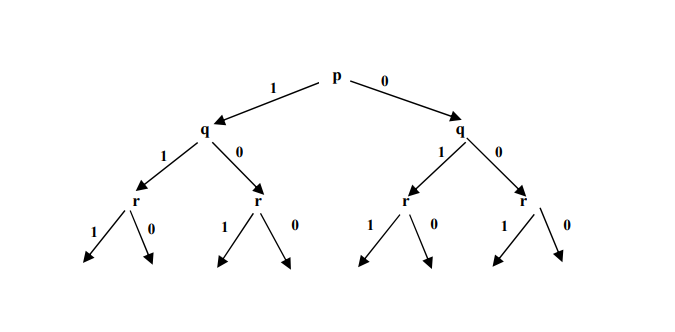
\includegraphics[width=0.8\textwidth]{Graphics/arboldp.png}
    \caption{Posible espacio de b\'usqueda de una FNC}
    \label{fig:arbol DP}
\end{figure}

\subsection{Davis-Putnam-Logemann-Loveland (DPLL)}
El algoritmo Davis-Putnam-Logemann-Loveland (DPLL) constituye una mejora significativa del método Davis-Putnam (DP), al preservar sus fundamentos teóricos y superar una de sus principales limitaciones: el consumo exponencial de memoria. Para ello, DPLL incorpora un mecanismo de retroceso (	extit{backtracking}) cronológico que le permite deshacer asignaciones al regresar al último nivel de decisión anterior una vez detectada una “cláusula de conflicto”ootnote{Se denomina cláusula de conflicto a aquella en la que todos sus literales son evaluados como falsos bajo una asignación parcial.}. Este enfoque permite explorar el árbol de búsqueda de forma más eficiente, reduciendo la necesidad de almacenar todas las ramas posibles.

DPLL adopta una estrategia de generación “lazy” del árbol de asignaciones: antes de realizar una nueva ramificación, verifica mediante propagación unitaria si existen conflictos que invaliden dicha extensión. Esta verificación garantiza que las asignaciones parciales se mantengan consistentes, y que las soluciones (cuando existen) se ubiquen en las hojas del árbol de decisión. En caso de que el conflicto se produzca en el nivel de decisión cero, y ambas asignaciones posibles para una variable hayan sido consideradas, se concluye que la fórmula es insatisfacible. En conjunto, el procedimiento de DPLL puede resumirse como una combinación de ramificación, propagación unitaria y retroceso sistemático.

Adicionalmente, DPLL incluye una etapa de preprocesamiento sobre la f\'ormula en Forma Normal Conjuntiva (FNC), en la cual se aplican simplificaciones basadas en leyes de la L\'ogica Proposicional. Entre estas se encuentra la eliminaci\'on de cl\'ausulas redundantes mediante el principio de subsunci\'on\footnote{Sean $C$ y $C'$ dos cl\'ausulas de una FNC; si $C' \subseteq C$, entonces $C'$ se considera subsumida por $C$ y puede eliminarse sin alterar la satisfacibilidad de la f\'ormula.}. Estas t\'ecnicas contribuyen a reducir el tama\~no de la instancia antes de la b\'usqueda propiamente dicha, mejorando la eficiencia del algoritmo sin comprometer su completitud.
Obsérvese el siguiente ejemplo:

Sea la FNC:

\begin{equation*}
\{\{\neg p,\neg q\},\{\neg p, \neg q\},\{\neg p,q,\neg r\},\{\neg p,r,s\},\{p,s\}\}
\end{equation*}

Simplificando mediante la ley de absorción:

\begin{equation*}
\{\{\neg p,\neg q\},\{\neg p,q,\neg r\},\{\neg p,r,s\},\{p,s\}\}
\end{equation*}

Eliminando el literal puro $s$:

\begin{equation*}
\{\{\neg p,\neg q\},\{\neg p,q,\neg r\}\}
\end{equation*}

Ramificando: $p = 1$

\begin{equation*}
\{\{\neg q\},\{q,\neg r\}\}
\end{equation*}

Aplicando \textbf{PU} en $\{\neg q\}$:

\begin{equation*}
\{\{\neg r\}\}
\end{equation*}

Aplicando \textbf{PU} en $\{\neg r\}$:

\begin{equation*}
\emptyset
\end{equation*}

Luego, la FNC es satisfacible.

No obstante la reducción del espacio de memoria de DPLL respecto a DP, aún persisten problemas fundamentales: la selección de variables, el \textit{backtrack} cronológico y la elección de cláusulas unitarias.

En primer lugar, la selección de la variable a la que se asignará un valor influye directamente en la ``forma'' del espacio de búsqueda. Una decisión inapropiada puede derivar en caminos significativamente más largos hacia una solución. Por tanto, resulta crucial emplear heurísticas que optimicen esta elección. (poner ejemplo)

En segundo lugar, el \textit{backtrack} cronológico ante un conflicto obliga a explorar, posiblemente de forma innecesaria, las asignaciones alternativas en niveles anteriores. Esta ineficiencia se acentúa cuando la causa real del conflicto se encuentra a $k$ niveles de distancia del punto donde se detectó. Además, DPLL no capitaliza las cláusulas que originaron los conflictos; es decir, no ``aprende'' de ellos. En consecuencia, es susceptible de incurrir reiteradamente en los mismos patrones erróneos de asignación.

Finalmente, el problema de la selección de cláusulas unitarias también repercute en la eficiencia del algoritmo, estando íntimamente relacionado con la estrategia de selección de variables.

\section{CDCL}
CDCL es una mejora que se le a\~nadi\'o al algoritmo DPLL con el objetivo de erradicar el problema del retroceso (\textit{backtrack}) cronol\'ogico, una vez encontrada una cl\'ausula de conflicto (todos sus literales eval\'uan 0).

El retroceso cronol\'ogico consiste en recorrer el \'arbol de decisi\'on (estructura propia del algoritmo DPLL que se forma al asignarle valores a las variables) retrocediendo de a 1 por cada nivel, probando todos los valores a\'un sin explorar de cada variable hasta encontrar la asignaci\'on causante del conflicto. Esta b\'usqueda es ineficiente dado que, adem\'as de analizar casos innecesarios, se vuelve susceptible a cometer el mismo error en el futuro (potencialmente realiza la misma combinaci\'on de asignaciones) generando b\'usquedas redundantes.

Para solucionar este problema, CDCL crea un grafo dirigido y ac\'iclico que permite guardar el historial de asignaciones de cada variable. En dicho grafo, los nodos son las variables y los arcos constituyen la causa de la asignaci\'on de dicha variable: la cl\'ausula a la que pertenece, si fue asignada por propagaci\'on unitaria, y \texttt{null} para variables asignadas por decisi\'on. El grafo tambi\'en contiene dos metadatos: el valor asignado a cada variable (0 o 1) y el nivel de decisi\'on en el que se asign\'o (los diferentes niveles de decisi\'on est\'an marcados por la asignaci\'on de valores por decisi\'on). Cabe destacar que la direcci\'on de los arcos en el grafo va desde las variables de decisi\'on hacia aquellas que, en el mismo nivel, tuvieron que forzar su valor por propagaci\'on unitaria. En el caso de una nueva variable de decisi\'on, se crea un nuevo arco con valor \texttt{null} desde la variable asignada por decisi\'on en el nivel anterior hasta la nueva variable.

Cuando una cl\'ausula resulta ser de conflicto (sus literales evaluaron 0), CDCL crea un nuevo nodo en el grafo que representa dicho conflicto, para comenzar con su an\'alisis. Este an\'alisis busca en el grafo la asignaci\'on causante del conflicto, para retroceder justo hacia ese punto y realizar un \textit{backjump} en lugar de un retroceso cronol\'ogico, como en DPLL. En caso de que el nivel del \textit{backjump} sea el nivel 0, CDCL considera la FNC como insatisfacible. Asimismo, con este an\'alisis CDCL busca conformar una cl\'ausula (cl\'ausula aprendida) que represente la combinaci\'on de asignaci\'on de valores que condujo a dicho conflicto, para incluirla en la base de datos de las cl\'ausulas de la FNC y evitar cometer el mismo error en iteraciones futuras. El punto escogido para realizar el \textit{backjump} es conocido como primer punto de implicaci\'on \'unico (\textit{First-UIP} por sus siglas en ingl\'es). Este punto ser\'a aquel literal que, en la cl\'ausula aprendida, posea el m\'as alto nivel de decisi\'on diferente del actual.

Es necesario enfatizar en el hecho de que la cl\'ausula aprendida debe contener \textbf{\'unicamente} un literal cuyo valor haya sido asignado en el nivel de decisi\'on actual. En caso de haber m\'as de uno, CDCL recorre el grafo en busca de la cl\'ausula que caus\'o la asignaci\'on de una de estas variables y aplica el Principio de Resoluci\'on entre esta y la cl\'ausula aprendida hasta el momento. La cl\'ausula resultante pasar\'a a ser la nueva cl\'ausula aprendida. El proceso se repetir\'a hasta que la cl\'ausula aprendida contenga solo un literal cuyo valor fue asignado en el nivel de decisi\'on actual.

A continuación, se muestra como ejemplo la implementación en Python de un CDCL SAT \textit{solver}

\begin{lstlisting}
class SATSolver:
    def __init__(self, formula):
        """
        Initializes the SAT solver.
        
        Parameters:
          formula: A list of clauses, where each clause is represented as a list of integers.
                   A positive integer i represents the variable x_i, and a negative integer -i represents -x_i.
        """
        # Copy the formula so that learned clauses can be appended.
        self.formula = formula[:]  
        self.assignments = {}    # Maps variable -> True/False assignment.
        self.levels = {}         # Maps variable -> decision level at which it was assigned.
        self.reasons = {}        # Maps variable -> clause that forced the assignment (None for decision variables).
        self.decision_level = 0  # Current decision level.
        self.decision_stack = [] # Stack storing tuples (variable, assigned value, decision level).

    def literal_value(self, literal):
        """
        Evaluates a literal given the current partial assignment.
        
        Returns:
          True if the literal is assigned True,
          False if the literal is assigned False,
          None if the variable is unassigned.
        """
        var = abs(literal)
        if var not in self.assignments:
            return None
        # For a positive literal, the assignment is the value; for a negative literal, invert the assignment.
        return self.assignments[var] if literal > 0 else not self.assignments[var]

    def check_clause(self, clause):
        """
        Determines the status of a clause with respect to current assignments.
        
        Returns a tuple (status, literal) where status is one of:
          - `satisfied': Clause is already True under the assignment.
          - `conflict': All literals are assigned False (the clause is unsatisfied).
          - `unit': Exactly one literal is unassigned while all others are False (this literal must be True).
          - `undefined': The clause is neither satisfied, conflicting, nor unit.
        """
        satisfied = False
        unassigned_count = 0
        unit_literal = None
        for literal in clause:
            val = self.literal_value(literal)
            if val is True:
                return (`satisfied', None)
            if val is None:
                unassigned_count += 1
                unit_literal = literal  # Last seen unassigned literal.
        if unassigned_count == 0:
            return (`conflict', None)
        if unassigned_count == 1:
            return (`unit', unit_literal)
        return (`undefined', None)

    def unit_propagate(self):
        """
        Repeatedly applies unit propagation.
        
        Returns:
          A conflicting clause if a conflict is found during propagation; otherwise, returns None.
        """
        changed = True
        while changed:
            changed = False
            for clause in self.formula:
                status, unit_literal = self.check_clause(clause)
                if status == 'conflict':
                    # A clause is unsatisfied => conflict!
                    return clause
                elif status == `unit':
                    var = abs(unit_literal)
                    if var not in self.assignments:
                        # Determine the value needed to satisfy the unit clause.
                        value = (unit_literal > 0)
                        self.assignments[var] = value
                        self.levels[var] = self.decision_level
                        self.reasons[var] = clause  # Store the clause as the reason for this assignment.
                        self.decision_stack.append((var, value, self.decision_level))
                        changed = True
        return None

    def pick_branching_variable(self):
        """
        Selects the next unassigned variable found in the formula.
        
        (In a production solver, better heuristics like VSIDS are used.)
        """
        variables = set()
        for clause in self.formula:
            for literal in clause:
                variables.add(abs(literal))
        for var in variables:
            if var not in self.assignments:
                return var
        return None

    def resolve(self, clause1, clause2, pivot):
        """
        Performs the resolution on two clauses over the pivot literal.
        
        Specifically, it returns:
          (clause1 \ {pivot}) U (clause2 \ {-pivot})
        """
        new_clause = []
        for lit in clause1:
            if lit == pivot:
                continue
            if lit not in new_clause:
                new_clause.append(lit)
        for lit in clause2:
            if lit == -pivot:
                continue
            if lit not in new_clause:
                new_clause.append(lit)
        return new_clause

    def conflict_analysis(self, conflict_clause): 
        """
        Conducts conflict analysis to find the First UIP.
        """
        learned_clause = conflict_clause.copy()
        current_level = self.decision_level

        while True:
            # Collect literals in the learned clause assigned at the current level
            current_level_lits = [
                lit for lit in learned_clause 
                if self.levels.get(abs(lit), -1) == current_level
            ]
            if len(current_level_lits) <= 1:
                break

            # Find the most recently assigned literal in current_level_lits
            last_literal = None
            # Iterate through assignments in reverse order (most recent first)
            for var, _, lvl in reversed(self.decision_stack):
                if lvl != current_level:
                    continue
                # Check if this variable is in current_level_lits
                for lit in current_level_lits:
                    if abs(lit) == var:
                        last_literal = lit
                        break
                if last_literal is not None:
                    break

            if last_literal is None:
                break  # No resolvable literals (should not happen)

            # Resolve with the reason clause of last_literal
            reason_clause = self.reasons.get(abs(last_literal))
            if reason_clause is None:
                break  # Decision literal; cannot resolve further

            learned_clause = self.resolve(learned_clause, reason_clause, last_literal)

        # Determine the backjump level
        backjump_level = 0
        for lit in learned_clause:
            lvl = self.levels.get(abs(lit), 0)
            if lvl != current_level and lvl > backjump_level:
                backjump_level = lvl

        return learned_clause, backjump_level

    def backjump(self, level):
        """
        Backtracks the search to the given decision level by undoing assignments above that level.
        """
        new_stack = []
        for var, value, lvl in self.decision_stack:
            if lvl > level:
                if var in self.assignments:
                    del self.assignments[var]
                if var in self.levels:
                    del self.levels[var]
                if var in self.reasons:
                    del self.reasons[var]
            else:
                new_stack.append((var, value, lvl))
        self.decision_stack = new_stack

    def solve(self):
        """
        The main solving loop which alternates between unit propagation, conflict analysis, and branching.
        
        Returns:
          A satisfying assignment as a dictionary mapping variables to Boolean values if the formula is SAT;
          Otherwise, returns None indicating the formula is UNSAT.
        """
        while True:
            conflict = self.unit_propagate()
            if conflict:
                if self.decision_level == 0:
                    # Conflict at level 0 indicates an unsolvable (UNSAT) condition.
                    return None
                learned_clause, backjump_level = self.conflict_analysis(conflict)
                # Learn the clause by adding it to the formula.
                self.formula.append(learned_clause)
                # Backjump to the appropriate decision level.
                self.backjump(backjump_level)
                self.decision_level = backjump_level
            else:
                var = self.pick_branching_variable()
                if var is None:
                    return self.assignments
                self.decision_level += 1
                # For this example, we simply decide that the variable is True.
                self.assignments[var] = True
                self.levels[var] = self.decision_level
                self.reasons[var] = None  # Decision assignments have no reason clause.
                self.decision_stack.append((var, True, self.decision_level))
\end{lstlisting}

La implementación anterior consiste en una clase \texttt{SATSolver} que realiza los pasos del algoritmo CDCL, dada una FNC escrita como un \textit{array} de \textit{arrays}, donde estos últimos representan las cláusulas. Cada variable está representada por un número entero positivo, y sus literales son ese número o su opuesto (negado).

El método \texttt{\_\_init\_\_(self, formula)} inicializa las estructuras internas:
\begin{itemize}
  \item \texttt{assignments}: Mapea cada variable con su valor asignado (\texttt{True} o \texttt{False}).
  \item \texttt{levels}: Mapea cada variable con el nivel de decisión en que fue asignada.
  \item \texttt{reasons}: Mapea cada variable con la cláusula que forzó su asignación, o \texttt{None} si fue por decisión. Estos funcionan como los ``arcos'' del grafo de decisión.
  \item \texttt{decision\_level}: Guarda el nivel actual de decisión.
  \item \texttt{decision\_stack}: Pila que registra el historial de asignaciones como tuplas: (variable, valor, nivel de decisión).
\end{itemize}

El bucle principal del algoritmo se encuentra en el método \texttt{solve(self)}. Mientras no se detecte un conflicto, asigna valores a variables no asignadas, actualizando las estructuras del solver. Si no quedan variables por asignar, devuelve la asignación completa y declara la fórmula como satisfacible. Si se detecta una cláusula conflicto y el nivel actual de decisión es 0, entonces devuelve \texttt{None}, declarando que la fórmula es insatisfacible. 

El método \texttt{unit\_propagate(self)} realiza propagación unitaria dentro de un ciclo de punto fijo que se repite mientras haya cambios (es decir, mientras existan cláusulas unitarias). Si se encuentra una cláusula conflicto, se detiene y la devuelve. Si no hay conflicto, retorna \texttt{None}. Para determinar el estado de una cláusula (\texttt{'satisfied'}, \texttt{'conflict'}, \texttt{'unit'}, \texttt{'undefined'}), se utiliza el método \texttt{check\_clause(self, clause)}.

Cuando se detecta una cláusula conflicto, se invoca \texttt{conflict\_analysis(self, conflict\_clause)}. Este analiza cuántos literales de la cláusula conflicto fueron asignados en el nivel de decisión actual. La cláusula aprendida debe contener exactamente un literal asignado en ese nivel. Si hay más de uno, se identifica el último literal asignado (según el grafo de decisión), se busca la cláusula que causó su asignación y se aplica el Principio de Resolución entre ella y la cláusula aprendida. Este proceso se repite hasta obtener una cláusula con un solo literal en el nivel actual.

Luego, se determina el \textit{backjump level}, es decir, el nivel de decisión más alto presente en los literales de la cláusula aprendida (distinto del actual). Si este nivel es 0, CDCL considera la FNC como insatisfacible. Finalmente, se invoca el método \texttt{backjump(self, level)} que deshace las asignaciones por encima del nivel objetivo y actualiza las estructuras correspondientes.


\section{DLIS}

La heur\'istica \textit{Dynamic Largest Individual Sum} (DLIS) es un m\'etodo aproximado de selecci\'on de variables que puede integrarse en un SAT \textit{solver} con CDCL, con el objetivo de mejorar la eficiencia al decidir qu\'e variable asignar en cada nivel de decisi\'on.

DLIS mantiene un contador por cada variable que indica la m\'axima cantidad de cl\'ausulas actualmente insatisfechas que podr\'ian satisfacerse al asignarle uno de sus dos posibles valores (0 o 1). Es decir, para una variable $x$, se calcula la cantidad de cl\'ausulas no satisfechas en las que aparece el literal $x$ (forma positiva) y su complemento $\neg x$ (forma negativa). Denotamos:

\begin{itemize}
  \item $\textit{count\_pos}(x)$: cantidad de veces que $x$ aparece positivamente en cl\'ausulas insatisfechas.
  \item $\textit{count\_neg}(x)$: cantidad de veces que $\neg x$ aparece en cl\'ausulas insatisfechas.
  \item $\textit{dlis}(x) = \max(\textit{count\_pos}(x), \textit{count\_neg}(x))$.
\end{itemize}

La pr\'oxima variable a seleccionar ser\'a aquella que maximice el valor de $\textit{dlis}(x)$ entre todas las variables no asignadas:

\begin{equation*}
  x_k \mid \textit{dlis}(x_k) = \max(\textit{dlis}(x_i)),\quad i \in [1,n]
\end{equation*}

donde $n$ es el total de variables de la FNC.

Obs\'ervese que si $\textit{count\_pos}(x_k) > \textit{count\_neg}(x_k)$, entonces se asigna a $x_k$ el valor 1; en caso contrario, se asigna 0. Esto con el objetivo de satisfacer la mayor cantidad de cl\'ausulas posibles en esa decisi\'on. El c\'alculo debe aplicarse \textbf{solo a las variables no asignadas} y \textbf{solo considerar valores a\'{u}n no explorados en el nivel actual de decisi\'on}.

Esta estrategia de selecci\'on de variables puede integrarse en el algoritmo CDCL previamente presentado, sustituyendo la funci\'on \texttt{pick\_branching\_variable(self)} por una versi\'on que implemente la heur\'istica DLIS.

A continuaci\'on, se presenta una posible implementaci\'on de esta heur\'istica, considerando como base el c\'odigo del \texttt{SATSolver} previamente desarrollado.

\begin{lstlisting}
def pick_branching_variable(self):
    """
    Selects the next unassigned variable using the DLIS heuristic.
    Returns (variable, value) to assign, or None if all variables are assigned.
    """
    pos_counts = {}
    neg_counts = {}
    # Count occurrences in unsatisfied clauses
    for clause in self.formula:
        status, _ = self.check_clause(clause)
        if status == 'satisfied':
            continue
        for lit in clause:
            var = abs(lit)
            if var not in self.assignments:
                if lit > 0:
                    pos_counts[var] = pos_counts.get(var, 0) + 1
                else:
                    neg_counts[var] = neg_counts.get(var, 0) + 1
    # Collect all variables in the formula to find unassigned ones not in any clause
    all_vars = set()
    for clause in self.formula:
        for lit in clause:
            all_vars.add(abs(lit))
    unassigned_vars = [var for var in all_vars if var not in self.assignments]
    if not unassigned_vars:
        return None
    # For variables not in pos/neg counts, set counts to 0
    for var in unassigned_vars:
        if var not in pos_counts:
            pos_counts[var] = 0
        if var not in neg_counts:
            neg_counts[var] = 0
    # Score variables based on DLIS heuristic
    scores = []
    for var in unassigned_vars:
        pos = pos_counts[var]
        neg = neg_counts[var]
        max_count = max(pos, neg)
        total = pos + neg
        scores.append((-max_count, -total, var))  # Negative for ascending sort
    scores.sort()  # Sorts by max_count (desc), then total (desc), then var (asc)
    var = scores[0][2]
    value = pos_counts[var] > neg_counts[var]
    return (var, value)

\end{lstlisting}

Las estructuras \texttt{pos\_counts} y \texttt{neg\_counts} se utilizan para almacenar, respectivamente, la cantidad de veces que el literal positivo y el literal negativo de cada variable no asignada aparece en las cláusulas actualmente insatisfechas. Este conteo es esencial para aplicar la heurística DLIS (\textit{Dynamic Largest Individual Sum}) de forma efectiva.

El procedimiento comienza recorriendo todas las cláusulas de la fórmula. Por cada cláusula que no esté satisfecha, se inspeccionan sus literales, y se incrementa el contador correspondiente de cada literal no asignado. Por ejemplo, si un literal positivo $x$ aparece en una cláusula insatisfecha, se incrementa \texttt{pos\_counts[$x$]}, y si aparece su complemento $\neg x$, se incrementa \texttt{neg\_counts[$x$]}.

Luego de este recorrido, se identifican todas las variables no asignadas que podrían no haber sido contadas, ya que podrían aparecer solamente en cláusulas ya satisfechas. A estas variables se les inicializa ambos contadores (positivo y negativo) en cero para garantizar una evaluación completa.

A continuación, se calcula el \textit{score} para cada variable no asignada, definido como el máximo entre \texttt{pos\_counts[$x$]} y \texttt{neg\_counts[$x$]}. Este valor representa la cantidad máxima de cláusulas que podrían satisfacerse al asignarle a la variable el valor correspondiente. Las variables se ordenan según su \textit{score} en orden descendente, y se elige aquella con el \textit{score} más alto como la próxima variable a asignar. En caso de empate, se utilizan criterios secundarios como la suma total de apariciones y el índice de la variable.

El valor que se asigna a la variable seleccionada depende de cuál de los dos conteos es mayor. Si \texttt{pos\_counts[$x$]} es mayor que \texttt{neg\_counts[$x$]}, entonces se asigna el valor \texttt{True} (es decir, $x$), de lo contrario se asigna \texttt{False} (es decir, $\neg x$).

Esta heurística DLIS tiene como objetivo maximizar el número de cláusulas satisfechas con cada asignación, lo que en teoría podría reducir la cantidad total de decisiones requeridas para encontrar una solución o para detectar una contradicción. Sin embargo, su aplicación resulta costosa para instancias de gran tamaño, debido a que implica una revisión completa de todas las cláusulas insatisfechas en cada nivel de decisión. Esto conduce a una complejidad computacional de $O(n)$ por nivel, donde $n$ es el número total de literales en la fórmula.

\section{VSIDS}

Por su parte, la heurística \textit{Variable State Independent Decaying Sum} (VSIDS) prioriza asignar valores a aquellas variables cuyos literales hayan estado involucrados en conflictos recientes. Para ello, VSIDS mantiene un \textit{score} para cada literal \( l \) (no por variable) que se incrementa cada vez que dicho literal aparece en cláusulas aprendidas a partir de conflictos. 

Además, para evitar que literales involucrados en conflictos antiguos tengan mayor prioridad que los relacionados con conflictos recientes, cada cierta cantidad \( T \) de conflictos se actualizan los \textit{scores} de todos los literales multiplicándolos por un factor de decaimiento \(\alpha\), con \(0 < \alpha < 1\) (usualmente \(\alpha = 0.95\)). 

Integrado en el algoritmo CDCL, VSIDS funciona del siguiente modo:

\begin{enumerate}
    \item Se ejecuta el algoritmo CDCL.
    \item Si ocurre un conflicto, se añade la cláusula aprendida \(\mathbf{C_{learn}}\). Luego, para cada literal \( l \) en \(\mathbf{C_{learn}}\), se actualiza su \textit{score} con \(score(l) = score(l) + \delta\), donde \(\delta\) es un incremento positivo.
    \item Si se alcanza el conflicto número \( T \), se actualiza el incremento con \( \delta = \delta \times \alpha \), con \(0 < \alpha < 1\).
    \item Si no ocurre un conflicto, se selecciona la variable \( v \) cuyo literal \( l_v \) cumple que su \textit{score} es máximo entre todos los literales \( l_i \), con \( i = 1, 2, \ldots, 2n \), siendo \( n \) la cantidad de variables. Si \( l_v \) es positivo, se asigna el valor 1 a \( v \), y 0 en caso contrario.
\end{enumerate}

\begin{lstlisting}
def pick_branching_variable(self):
    """
    Selects the next unassigned variable using the VSIDS heuristic (highest activity).
    """
    candidates = []
    for var in self.activity:
        if var not in self.assignments:
            candidates.append(var)
    if not candidates:
        return None
    # Select the candidate with the highest activity; in case of tie, choose the smallest variable.
    max_activity = max(self.activity[var] for var in candidates)
    best_vars = [var for var in candidates if self.activity[var] == max_activity]
    best_vars.sort()  # Deterministic tie-breaking by choosing the smallest variable
    return best_vars[0]
\end{lstlisting}

Este método selecciona, de entre las variables aún no asignadas, aquella con el mayor \textit{score} de acuerdo con la estrategia VSIDS. Para implementar este comportamiento, se añade a la clase \textit{SATSolver} una estructura llamada \textit{activity}, la cual asocia a cada variable un valor numérico que representa su actividad o relevancia. Esta estructura se inicializa al comienzo de la ejecución inspeccionando todas las variables presentes en las cláusulas de la fórmula, como se muestra a continuación:

\begin{lstlisting}
# previus code
    for clause in self.formula:
        for lit in clause:
            var = abs(lit)
            if var not in self.activity:
                self.activity[var] = 0.0
\end{lstlisting}

Durante la ejecución del algoritmo CDCL, la estructura \textit{activity} se actualiza dentro del método \textit{solve(self)}. En particular, cada vez que se detecta un conflicto y se aprende una nueva cláusula, se incrementa la actividad de todas las variables que aparecen en dicha cláusula. Además, para priorizar los conflictos más recientes, se aplica un factor de decaimiento a todas las variables. A continuación se muestra el fragmento correspondiente:

\begin{lstlisting}
decay_factor = 0.95
while True:
    conflict = self.unit_propagate()
    if conflict:
        if self.decision_level == 0:
            # Conflict at level 0 indicates an unsolvable (UNSAT) condition.
            return None
        learned_clause, backjump_level = self.conflict_analysis(conflict)
        # Learn the clause by adding it to the formula.
        self.formula.append(learned_clause)
        # Update activities for variables in the learned clause
        for lit in learned_clause:
            var = abs(lit)
            self.activity[var] += 1.0
        # Decay all activities
        for var in self.activity:
            self.activity[var] *= decay_factor
        # Backjump to the appropriate decision level.
        self.backjump(backjump_level)
        self.decision_level = backjump_level
# rest of code
\end{lstlisting}

De este modo, la heurística VSIDS logra priorizar variables relevantes en conflictos recientes, mejorando la toma de decisiones del solucionador sin necesidad de reexaminar toda la fórmula.


\section{Reinicio (\textit{restart})}

Las estrategias de reinicio tienen como objetivo evitar que el algoritmo de CDCL se estanque en regiones locales del espacio de búsqueda. Para ello, se permite reiniciar el árbol de decisiones, es decir, eliminar todas las asignaciones realizadas hasta el momento y comenzar nuevamente desde el nivel de decisión cero. Sin embargo, se conservan las cláusulas aprendidas durante el proceso, así como la información acumulada por las heurísticas de selección de variables (por ejemplo, las actividades de los literales en VSIDS o los conteos en DLIS).

Estas estrategias buscan que, al conservar el conocimiento adquirido (cláusulas aprendidas), el solucionador pueda explorar regiones más prometedoras del espacio de soluciones sin tener que recorrer nuevamente caminos improductivos.

Existen diversos criterios para decidir cuándo realizar un reinicio:

\begin{enumerate}
    \item \textbf{Fijo}: se realiza un reinicio después de un número fijo $k$ de conflictos. Esta es una estrategia sencilla pero poco adaptativa.

    \item \textbf{Geométrico}: el número de conflictos entre reinicios crece de forma geométrica según la relación $r_0 = b$, $r_i = \alpha \cdot r_{i-1}$ con $\alpha > 1$. Esta estrategia permite reinicios más frecuentes al principio, reduciéndose con el tiempo. Un valor muy grande de $\alpha$ puede hacer que los reinicios sean demasiado esporádicos, mientras que un valor muy pequeño puede provocar una sobrecarga de reinicios.

    \item \textbf{Luby}: utiliza la secuencia de Luby $(1,1,2,1,1,2,4,1,1,2,\dots)$ para definir los intervalos entre reinicios, según la fórmula $r_i = b \cdot \text{Luby}(i)$, donde $b$ es un parámetro base que define el tamaño mínimo del intervalo. Esta estrategia tiene fundamentos teóricos que justifican su uso en entornos donde no se conoce a priori una buena política de reinicio.

    \item \textbf{Glucose-style (basada en LBD)}: esta estrategia se basa en el cómputo de la medida Literal Block Distance (LBD) de las cláusulas aprendidas. Dada una cláusula $C_{learn}$, su LBD se define como el número de niveles de decisión distintos a los que pertenecen sus literales:
    \begin{equation*}
        \text{LBD}(C_{learn}) = |\{ \text{level}(l)\mid l \in C_{learn} \}|
    \end{equation*}
    La idea es que una cláusula con menor LBD involucra decisiones más cercanas entre sí, lo que la hace más relevante para guiar el proceso de resolución. 

    Para implementar esta estrategia, se mantienen dos promedios móviles de los LBD: uno para una ventana rápida de conflictos recientes (por ejemplo, los últimos 50 o 100) y otro para una ventana más larga (por ejemplo, los últimos 1000). Denotando estos promedios como $\mu_r$ (rápido) y $\mu_l$ (lento), se define un umbral $T > 1$. Si se cumple la condición:
    \begin{equation*}
        \frac{\mu_r}{\mu_l} > T
    \end{equation*}
    entonces se considera que el solucionador está atrapado en una región poco productiva y se procede con un reinicio.
\end{enumerate}

La incorporación de estrategias de reinicio, particularmente aquellas adaptativas como Luby o Glucose-style, ha demostrado ser fundamental para el éxito de solucionadores modernos de SAT, ya que permiten alternar entre exploración y explotación de manera eficiente en espacios de búsqueda complejos.

Ussando como base el código anterior de CDCL, una posible implementación para la estrategia Luby puede ser la siguiente:

\begin{lstlisting}
# restart_luby.py

from collections import deque

def luby(u, k):
    """
    Generates the k-th value of the Luby sequence multiplied by u (unit run).
    """
    def _luby(i):
        # Encuentra el mayor j tal que i = 2^j - 1
        j = 1
        while (1 << j) - 1 < i:
            j += 1
        if i == (1 << j) - 1:
            return 1 << (j - 1)
        return _luby(i - (1 << (j - 1)) + 1)
    return u * _luby(k)

class SATSolverLuby:
    def __init__(self, formula, unit_run=100):
        from restart_luby import luby  # si ejecutas desde fuera
        self.formula = formula[:]  
        self.assignments = {}
        self.levels = {}
        self.reasons = {}
        self.decision_level = 0
        self.decision_stack = []
        # Luby restart parameters
        self.unit_run = unit_run
        self.luby_idx = 1
        self.conflicts_since_restart = 0
        self.next_restart = luby(self.unit_run, self.luby_idx)

    # the same functions (literal_value, check_clause, unit_propagate,
    # pick_branching_variable, resolve, conflict_analysis, backjump)

    def solve(self):
        while True:
            conflict = self.unit_propagate()
            if conflict:
                self.conflicts_since_restart += 1
                if self.decision_level == 0:
                    return None
                learned_clause, backjump_level = self.conflict_analysis(conflict)
                self.formula.append(learned_clause)
                self.backjump(backjump_level)
                self.decision_level = backjump_level

                # restart?
                if self.conflicts_since_restart >= self.next_restart:
                    # Restart: clear assignments, preserve learned clauses
                    self.assignments.clear()
                    self.levels.clear()
                    self.reasons.clear()
                    self.decision_stack.clear()
                    self.decision_level = 0
                    # Prepare next umbral
                    self.luby_idx += 1
                    self.next_restart = luby(self.unit_run, self.luby_idx)
                    self.conflicts_since_restart = 0
            else:
                var = self.pick_branching_variable()
                if var is None:
                    return self.assignments
                self.decision_level += 1
                self.assignments[var] = True
                self.levels[var] = self.decision_level
                self.reasons[var] = None
                self.decision_stack.append((var, True, self.decision_level))
\end{lstlisting}

En el caso de la estrategia basada en la secuencia de Luby, esta se ha integrado al algoritmo CDCL modificando su estructura de control de conflictos. Para ello, se define una funci\'on \texttt{luby(u, k)} que genera el k-\'esimo valor de la secuencia de Luby multiplicado por una unidad base \texttt{u}, la cual determina el n\'umero de conflictos que deben ocurrir antes de realizar un reinicio.

Dentro de la clase principal del solucionador, se inicializan los siguientes parámetros:

\begin{itemize}
    \item \texttt{unit\_run}: intervalo base de conflictos entre reinicios.
    \item \texttt{luby\_idx}: índice actual dentro de la secuencia de Luby.
    \item \texttt{conflicts\_since\_restart}: contador de conflictos desde el último reinicio.
    \item \texttt{next\_restart}: umbral de conflictos para el siguiente reinicio, calculado como \texttt{luby(unit\_run, luby\_idx)}.
\end{itemize}

Durante la ejecución del método \texttt{solve()}, cada vez que se detecta un conflicto y se realiza el correspondiente análisis y retroceso (“\textit{backjump}”), se incrementa el contador de conflictos. Luego, se verifica si el número acumulado de conflictos ha alcanzado el umbral definido por la secuencia de Luby. En caso afirmativo, se ejecuta un reinicio que implica:

\begin{itemize}
    \item Vaciar las estructuras de asignaciones, niveles de decisión, razones de propagación y la pila de decisiones.
    \item Reiniciar el nivel de decisión a cero.
    \item Calcular el nuevo umbral de reinicio actualizando el índice de Luby y recalculando \texttt{next\_restart}.
    \item Reiniciar el contador de conflictos desde el reinicio.
\end{itemize}

Cabe destacar que durante el reinicio no se eliminan las cláusulas aprendidas, lo cual permite conservar información valiosa obtenida en decisiones anteriores. Esta estrategia favorece la salida de áreas del espacio de búsqueda poco prometedoras, maximizando la posibilidad de encontrar una solución en regiones más relevantes del espacio de soluciones.


De igual modo, una implementación para la estrategia \textit{Glucose-Style (LBD-based)} sería como la que se muestra a continuación:

\begin{lstlisting}
# restart_glucose.py

class SATSolverGlucose:
    def __init__(self, formula, lbd_window=50):
        self.formula = formula[:]  
        self.assignments = {}
        self.levels = {}
        self.reasons = {}
        self.decision_level = 0
        self.decision_stack = []
        # Glucose-style parameters
        self.lbd_history = []
        self.window_size = lbd_window
        self.prev_avg_lbd = float('inf')

    #same base functions: literal_value, check_clause, unit_propagate, pick_branching_variable, resolve, backjump

    def conflict_analysis(self, conflict_clause):
        learned_clause, backjump_level = super().conflict_analysis(conflict_clause)
        # Calcular LBD (Literal Block Distance)
        levels = { self.levels.get(abs(l), 0) for l in learned_clause }
        lbd = len(levels)
        # Mantener ventana de LBDs
        self.lbd_history.append(lbd)
        if len(self.lbd_history) > self.window_size:
            self.lbd_history.pop(0)
        return learned_clause, backjump_level

    def should_restart(self):
        if len(self.lbd_history) < self.window_size:
            return False
        curr_avg = sum(self.lbd_history) / len(self.lbd_history)
        # Reiniciar si la media de LBD sube respecto al ciclo anterior
        if curr_avg > self.prev_avg_lbd:
            self.prev_avg_lbd = curr_avg
            return True
        self.prev_avg_lbd = curr_avg
        return False

    def solve(self):
        while True:
            conflict = self.unit_propagate()
            if conflict:
                if self.decision_level == 0:
                    return None
                learned_clause, backjump_level = self.conflict_analysis(conflict)
                self.formula.append(learned_clause)
                self.backjump(backjump_level)
                self.decision_level = backjump_level

                # Glucose-style restart
                if self.should_restart():
                    self.assignments.clear()
                    self.levels.clear()
                    self.reasons.clear()
                    self.decision_stack.clear()
                    self.decision_level = 0

            else:
                var = self.pick_branching_variable()
                if var is None:
                    return self.assignments
                self.decision_level += 1
                self.assignments[var] = True
                self.levels[var] = self.decision_level
                self.reasons[var] = None
                self.decision_stack.append((var, True, self.decision_level))

\end{lstlisting}

\section{Selecci\'on de cl\'ausulas unitarias}

Una de las estrategias m\'as empleadas en solucionadores modernos de SAT para optimizar la propagaci\'on unitaria es \\textit{Two Watched Literals (TWL)}. Esta t\'ecnica tiene como objetivo evitar el recorrido exhaustivo de todas las cl\'ausulas en cada paso de propagaci\'on, mediante la vigilancia de dos literales por cl\'ausula, denominados $l_1$ y $l_2$.

Durante la ejecuci\'on del algoritmo, si ambos literales vigilados en una cl\'ausula no han sido evaluados, o al menos uno de ellos tiene valor verdadero, entonces no es necesario revisar dicha cl\'ausula, ya que no es unitaria ni entra en conflicto. En caso contrario, si uno de los literales es asignado a falso, se intenta buscar dentro de la cl\'ausula otro literal que no haya sido evaluado o que tenga valor verdadero, con el fin de reemplazar al literal que fue asignado a falso. Si no se encuentra un reemplazo v\'alido y el otro literal vigilado a\'un no tiene valor, entonces la cl\'ausula se vuelve unitaria, forzando la asignaci\'on del segundo literal. Si ambos literales vigilados son evaluados a falso, la cl\'ausula se considera en conflicto.

Esta estrategia resulta altamente eficiente, ya que disminuye considerablemente el n\'umero de cl\'ausulas que deben revisarse en cada nivel de decisi\'on, optimizando as\'i el rendimiento del algoritmo CDCL.

Para integrar la estrategia TWL en el c\'odigo base de CDCL, es necesario modificar la estructura interna del solucionador, incluyendo los m\'etodos de propagaci\'on, asignaci\'on y retroceso, entre otros. A continuaci\'on se presentar\'a un ejemplo de implementaci\'on.

%\begin{lstlisting}
%import formulas as f
%from collections import defaultdict, deque
%
%class SATSolver:
%    def __init__(self, formula):
%        """
%        Initializes the SAT solver.
%
%        Parameters:
%          formula: A list of clauses, where each clause is represented as a list of integers.
%                   A positive integer i represents the variable x_i, and a negative integer -i represents -x_i.
%        """
%        # Copy the formula so that learned clauses can be appended.
%        self.clauses = [list(c) for c in formula]
%        self.assignments = {}    # Maps variable -> True/False assignment.
%        self.levels = {}         # Maps variable -> decision level at which it was assigned.
%        self.reasons = {}        # Maps variable -> clause that forced the assignment (None for decision vars).
%        self.decision_level = 0  # Current decision level.
%        self.decision_stack = [] # Stack of (variable, value, level).
%
%        # Two-Watched Literals: map literal -> list of clause indices watching it
%        self.watches = defaultdict(list)
%        self._init_watches()
%
%    def _init_watches(self):
%        """Initialize two watched literals per clause."""
%        for ci, clause in enumerate(self.clauses):
%            # If clause has only one literal, watch it twice.
%            w0 = clause[0]
%            w1 = clause[1] if len(clause) > 1 else clause[0]
%            self.watches[w0].append(ci)
%            self.watches[w1].append(ci)
%
%    def literal_value(self, literal):
%        """
%        Evaluate a literal under current partial assignment.
%        Returns True, False, or None if unassigned.
%        """
%        var = abs(literal)
%        if var not in self.assignments:
%            return None
%        return self.assignments[var] if literal > 0 else not self.assignments[var]
%
%    def check_clause(self, clause):
%        """
%        Determine clause status: 'satisfied', 'conflict', 'unit', or 'undefined'.
%        If 'unit', also return the unit literal.
%        """
%        unassigned = 0
%        last = None
%        for lit in clause:
%            val = self.literal_value(lit)
%            if val is True:
%                return ('satisfied', None)
%            if val is None:
%                unassigned += 1
%                last = lit
%        if unassigned == 0:
%            return ('conflict', None)
%        if unassigned == 1:
%            return ('unit', last)
%        return ('undefined', None)
%
%    def _enqueue(self, var, value, level, reason):
%        """
%        Assign var=value at given level with reason and push onto decision stack.
%        Returns the corresponding literal for propagation.
%        """
%        self.assignments[var] = value
%        self.levels[var] = level%
%        self.reasons[var] = reason%
%        self.decision_stack.append((var, va%lue, level))
%        return var if value else -var%
%
%    def unit_propagate(self):%
%        """%
%        Perform unit propagation using two-%watched literals.
%        Returns a conflicting clause if con%flict, else None.
%        """%
%        queue = deque()%
%        # Enqueue all literals assigned at %current level
%        for var, val, lvl in self.decision_%stack:
%            if lvl == self.decision_level:%
%                queue.append(var if val els%e -var)
%
%        while queue:%
%            lit = queue.popleft()%
%            lit_false = -lit%
%            # We iterate over a snapshot si%nce watch list may change
%            watchers = list(self.watches[li%t_false])
%            for ci in watchers:%
%                clause = self.clauses[ci]%
%                # Try to find a new literal% to watch instead of lit_false
%                found_replacement = False%
%                for l in clause:%
%                    if l == lit_false:%
%                        continue%
%                    if self.literal_value(l%) is not False:
%                        # relocate watch fr%om lit_false to l
%                        self.watches[l].app%end(ci)
%                        self.watches[lit_fa%lse].remove(ci)
%                        found_replacement =% True
%                        break%
%                if found_replacement:%
%                    continue%
%
%                # No replacement found: cla%use must be unit or conflict
%                status, unit_lit = self.che%ck_clause(clause)
%                if status == 'conflict':%
%                    return clause%
%                elif status == 'unit':%
%                    v = abs(unit_lit)%
%                    if v not in self.assign%ments:
%                        new_lit = self._enq%ueue(v, unit_lit > 0, self.decision_level, clause)
%                        queue.append(new_li%t)
%        return None%
%
%    def pick_branching_variable(self):%
%        """%
%        Select next unassigned variable (na%ive).
%        """%
%        all_vars = {abs(l) for c in self.cl%auses for l in c}
%        for v in all_vars:%
%            if v not in self.assignments:%
%                return v%
%        return None%
%
%    def resolve(self, c1, c2, pivot):%
%        """%
%        Resolve two clauses on pivot litera%l.
%        Returns the resolvent.%
%        """%
%        res = [l for l in c1 if l != pivot]%
%        for l in c2:%
%            if l != -pivot and l not in res%:
%                res.append(l)%
%        return res%
%
%    def conflict_analysis(self, conflict_clause):
%        """
%        First-UIP conflict analysis.
%        Returns (learned_clause, backjump_level).
%        """
%        learned = conflict_clause.copy()
%        cur_lvl = self.decision_level
%        while True:
%            # Count lits at current level
%            lvl_lits = [l for l in learned if self.levels.get(abs(l), -1) == cur_lvl]
%            if len(lvl_lits) <= 1:
%                break
%            # Find most recent one
%            last = None
%            for v,_,lvl in reversed(self.decision_stack):
%                if lvl != cur_lvl:
%                    continue
%                for l in lvl_lits:
%                    if abs(l) == v:
%                        last = l
%                        break
%                if last:
%                    break
%            reason = self.reasons.get(abs(last))
%            if not reason:
%                break
%            learned = self.resolve(learned, reason, last)
%
%        # Compute backjump level
%        back_lvl = 0
%        for l in learned:
%            lvl = self.levels.get(abs(l), 0)
%            if lvl != cur_lvl and lvl > back_lvl:
%                back_lvl = lvl
%        return learned, back_lvl
%
%    def backjump(self, level):
%        """
%        Undo assignments above given level.
%        """
%        new_stack = []
%        for v, val, lvl in self.decision_stack:
%            if lvl > level:
%                self.assignments.pop(v, None)
%                self.levels.pop(v, None)
%                self.reasons.pop(v, None)
%            else:
%                new_stack.append((v, val, lvl))
%        self.decision_stack = new_stack
%
%    def solve(self):
%        """
%        Main CDCL loop.
%        Returns a satisfying assignment or None if UNSAT.
%        """
%        while True:
%            conflict = self.unit_propagate()
%            if conflict:
%                if self.decision_level == 0:
%                    return None
%                learned, bj = self.conflict_analysis(conflict)
%                # add learned clause and set up its watches
%                self.clauses.append(learned)
%                ci = len(self.clauses) - 1
%                w0 = learned[0]
%                w1 = learned[1] if len(learned) > 1 else learned[0]
%                self.watches[w0].append(ci)
%                self.watches[w1].append(ci)
%                # backjump and continue
%                self.backjump(bj)
%                self.decision_level = bj
%            else:
%                var = self.pick_branching_variable()
%                if var is None:
%                    return self.assignments
%                # make a new decision
%                self.decision_level += 1
%                lit = self._enqueue(var, True, self.decision_level, None)
%\end{lstlisting}


La implementaci\'on del algoritmo CDCL puede enriquecerse significativamente mediante la integraci\'on de estrategias que optimicen sus componentes cr\'iticos. Una de estas mejoras es la adopci\'on del esquema Two Watched Literals (TWL), el cual transforma de manera sustancial la manera en que se gestiona la propagaci\'on unitaria.

En la versi\'on b\'asica de CDCL, el procedimiento de propagaci\'on unitaria examina exhaustivamente todas las cl\'ausulas de la f\'ormula para identificar aquellas que se reducen a una sola literal no asignada bajo la interpretaci\'on parcial actual. Este enfoque, si bien correcto, resulta ineficiente, ya que el costo computacional de revisar cl\'ausula por cl\'ausula crece linealmente con el tama\~no de la f\'ormula. En contraste, el enfoque basado en TWL introduce una estructura auxiliar que asigna a cada cl\'ausula exactamente dos literales que act\'uan como ``vigilantes''. Mientras al menos uno de ellos no est\'e asignado a falso, se garantiza que la cl\'ausula no puede causar conflicto ni ser unitaria, permitiendo as\'i omitir su revisi\'on durante la propagaci\'on.

El impacto de esta estrategia se observa de inmediato en la estructura del c\'odigo. En la implementaci\'on enriquecida, se incorpora un diccionario que mapea cada literal a una lista de \'indices de cl\'ausulas que lo est\'an ``observando''. Esta organizaci\'on permite que, ante la asignaci\'on de un literal, solo se revisen aquellas cl\'ausulas que lo tienen como vigilante, reduciendo de forma dr\'astica la cantidad de cl\'ausulas analizadas en cada nivel de decisi\'on. Adem\'as, se redefine el procedimiento de propagaci\'on unitaria para que, al detectar que un literal vigilado ha sido evaluado a falso, se intente encontrar otro literal en la cl\'ausula que pueda ocupar su lugar como nuevo vigilante. Si esto no es posible y el otro literal vigilado tampoco satisface la cl\'ausula, se deduce que esta es unitaria o de conflicto, y se act\'ua en consecuencia.

Adem\'as de modificar la propagaci\'on unitaria, la estrategia TWL afecta tambi\'en la gesti\'on de cl\'ausulas aprendidas. Cada vez que se genera una nueva cl\'ausula como resultado del an\'alisis de conflictos, se seleccionan dos de sus literales para ser vigilados y se actualizan las estructuras de observaci\'on en consecuencia. Esto asegura que las optimizaciones ofrecidas por TWL se mantengan vigentes incluso cuando la f\'ormula evoluciona durante la ejecuci\'on del algoritmo.

En s\'intesis, la transici\'on desde un esquema de propagaci\'on unitaria tradicional hacia un enfoque basado en Two Watched Literals representa una mejora sustancial en t\'erminos de eficiencia algor\'itmica. Al limitar el conjunto de cl\'ausulas a inspeccionar en cada paso, se logra una aceleraci\'on significativa del proceso de inferencia, lo cual resulta especialmente beneficioso en instancias de gran escala, donde los costos de propagaci\'on pueden dominar el tiempo total de ejecuci\'on. Esta adaptaci\'on no solo evidencia una comprensi\'on profunda de los mecanismos internos de CDCL, sino que tambi\'en refleja el compromiso con la incorporaci\'on de estrategias de vanguardia para la resoluci\'on eficiente del problema de satisfacibilidad booleana.
